\section{Annuli and charged-field estimates}\label{sec:annuli}

We now use the conformal net $A_V$ constructed in
Corollary~\ref{cor:locality}.  The purpose of this section is to obtain
analytic bounds for charged fields before constructing the net
representations associated to their target modules.  The source of a
charged field will initially be the vacuum module $V$.  More generally,
the argument works whenever its source module has already been integrated.
This order will allow us to prove integration before using positivity of
general fusion products.

\subsection{Localized annuli and their ranges}

We use the annulus constructions of Henriques--Tener
\cite{HTVirasoro,HTVOA,HTGenusZero}.  An annulus may have incoming and
outgoing boundaries that touch, but do not cross.  A lift of an annulus
means an element of the centrally extended covering semigroup
$\widetilde{\operatorname{Ann}}_c$, where $c$ is the central charge.
Lifts act by bounded operators in positive-energy unitary Virasoro
representations.  Gluing is multiplication, with the right factor acting
first, and reflection is denoted by $\dagger$ and acts by the Hilbert-space
adjoint.  On the grading-restricted unitary modules used below, fixed
lifted annuli and their adjoints preserve every energy Sobolev space and
hence the smooth domain continuously
\cite[Theorem~4.8, Remark~4.9 and Theorem~5.5]{HTVirasoro}.

The VOA reconstructed from $A_V$ is $V$ itself
\cite[Theorem~8.9(ii)]{HTVOA}.  Thus the point-insertion labels in that
construction are the vectors of $V$.  We write
$\underline A[v(z)]$ for an insertion with the standard local coordinate
$\zeta\mapsto z+\zeta$.  More generally, $p_*v(0)$ denotes the label
obtained by a change of local coordinate $p$; for
$p(\zeta)=z+q\zeta$, $q>0$, it is $(q^{L_0}v)(z)$.
Finite-energy labels are transported by the usual formal coordinate action.
Insertions compose under gluing and depend holomorphically on their
positions.  They also commute with reflection
\cite[Section~6 and Proposition~6.19]{HTVOA}.

For $0<\rho\leq1$ a smooth function on $S^1$, consider the radial annulus
whose incoming and outgoing parametrizations are
\[
 e^{i\vartheta}\longmapsto\rho(e^{i\vartheta})e^{i\vartheta},
 \qquad e^{i\vartheta}\longmapsto e^{i\vartheta}.
\]
If $1-\rho$ is compactly supported in an interval $I$, radial interpolation
gives a lift $\underline A$ localized in $I$.  Its vacuum operator belongs
to $A_V(I)$.  The same holds for its point insertions, and their actions
in a locally normal representation $\pi$ are their images under $\pi_I$
\cite[Lemma~6.8]{HTVOA}.  The reflected double
\[
 \widehat A=\underline A^\dagger\underline A
\]
can be drawn in the plane between the radial curves $\rho$ and
$\rho^{-1}$.  The two annuli meet along the unit circle.

The complementary-annulus argument below is the exact-preimage
argument of \cite[Lemma~7.9]{HTVOA}. We record its range and density
consequences in the form used for charged fields.

\begin{lemma}[Ranges of annulus operators]\label{lem:annulus-range}
Let $\underline A,\underline B$ be lifted annuli satisfying
$\underline A\underline B=s_0^{L_0}$, with $0<s_0<1$, in a
positive-energy representation with dense finite-energy subspace $E$.
Then
\[
 E\subset\operatorname{ran}\underline A,
 \qquad \underline A^{-1}E=\underline B E,
 \qquad \overline{\underline A^{-1}E}=\mathcal H.
\]
Every radial annulus above admits such a complementary factor
$\underline B$ when $s_0<\min\rho$.
\end{lemma}

\begin{proof}
The geometric complement between the circle of radius $s_0$ and the
incoming boundary gives $B$.  Choose its lift so that the product is the
standard lift of the round annulus; any necessary scalar and winding are
absorbed in this fixed choice.  Annulus operators are injective with
dense range \cite[Lemma~4.15]{HTVOA}.  Since $s_0^{L_0}$ is invertible on
$E$, its range contains $E$, and $\underline B E\subset
\underline A^{-1}E$.  Conversely, if $\underline A\xi\in E$, injectivity
of $\underline A$ gives
\[
 \xi=\underline B s_0^{-L_0}\underline A\xi\in\underline B E.
\]
Finally, $\underline B$ is bounded with dense range and $E$ is dense.
These observations also prove the assertion when the energy eigenspaces
are not finite dimensional; compare \cite[Lemma~7.9]{HTVOA}.
\end{proof}

Let $N$ be an already strongly integrable unitary $V$-module, with local
representations $\pi_I^N$.  Subscripts $N$ on annulus operators refer to
the resulting net representation.  The Virasoro action used here is the
module Virasoro action: the closed stress-energy smears agree by strong
integration, and a partition of unity identifies their modes, including
$L_0$.  The reconstructed module is consequently $N$, by the uniqueness
statement in \cite[Theorem~9.5(ii) and Corollary~9.6]{HTVOA}.
In particular, for the standard lifted round annulus with radii $s<R$,
\begin{equation}\label{eq:round-insertion}
 A_{R,s,N}[v(z)]=R^{-L_0}Y^N(v,z)s^{L_0}
\end{equation}
in finite-energy matrix coefficients.  For a radial annulus $A$ and
$z$ in its interior, gluing with the complementary factor in
Lemma~\ref{lem:annulus-range} gives
\begin{equation}\label{eq:annulus-insertion}
 \begin{split}
 \underline A_N[v(z)]\xi
   &=Y^N(v,z)\underline A_N\xi,\\
 \langle\widehat A_N[v(z)]\xi,\eta\rangle
   &=\langle Y^N(v,z)\underline A_N\xi,
                         \underline A_N\eta\rangle,
 \qquad \xi,\eta\in\underline A_N^{-1}N.
 \end{split}
\end{equation}
These are identities on the indicated exact dense preimages, rather than
identities of arbitrary products of unbounded operators.

\subsection{A fixed-disc estimate and a uniform round estimate}

\begin{lemma}[Insertion in a fixed disc]\label{lem:fixed-disc}
Let $\widehat A=\underline A^\dagger\underline A$ be a fixed localized
double, and let $S_0$ be a closed round disc strictly inside it.
There is a constant $C_{\widehat A,S_0}$ such that, for every Möbius
embedding $p:\mathbb D\to\mathring S_0$ and $v\in V$,
\begin{equation}\label{eq:fixed-disc-bound}
 \|\widehat A_N[p_*v(0)]\|
     \leq C_{\widehat A,S_0}\|v\|
\end{equation}
in every already integrated unitary module $N$.  Here $\mathbb D$ is the
closed unit disc, and embeddings are smooth up to their boundaries.
\end{lemma}

\begin{proof}
Write the underlying double as $D_{\rm out}\setminus
\mathring D_{\rm in}$.  The inclusion
$S_0\sqcup D_{\rm in}\to D_{\rm out}$ is a multidisc embedding: the
incoming closed discs are disjoint, although $D_{\rm in}$ may meet the
outgoing boundary.  The bounded map of
\cite[Theorem~A, or Theorem~3.6]{HTGenusZero} yields
\[
 H_0(S_0)\otimes H_0(D_{\rm in})\longrightarrow H_0(D_{\rm out}).
\]
Evaluating its first slot at an inserted vector, and using
\cite[Corollary~A.1]{HTGenusZero}, gives the corresponding inserted
annulus operator.  The boundary identification operators are unitary;
the scalar comparing the fixed lift with this vacuum map is independent
of the insertion \cite[Lemma~6.10]{HTVOA}.

Identify $S_0$ conformally with $\mathbb D$.  The resulting Möbius
embedding factors into disc automorphisms and a dilation of radius less
than one.  Its covered univalent lift acts by unitaries and a
positive-energy contraction.  The state associated to $p_*v(0)$ in
$H_0(S_0)$ therefore has norm at most $\|v\|$.  This proves the vacuum
bound.  The inserted vacuum operator belongs to $A_V(I)$ for the
localizing interval of the double.  Its image under $\pi_I^N$ is the
inserted operator on $N$; contractivity proves the same bound there.
\end{proof}

In particular, over a compact subarc on which $\rho<1$, put
\[
 \delta=|z|^{-1}-|z|,\qquad q=2\delta.
\]
For $|z|<1$ sufficiently close to one, the small disc
$z+q\mathbb D$ lies in one of finitely many fixed discs strictly inside
the double.  Lemma~\ref{lem:fixed-disc} is thus uniform for the labels
$(q^{L_0}v)(z)$ throughout that collar.  The next estimate supplies the
corresponding uniform control when both boundaries are round and shrink
towards the insertion.  A bound for each fixed annulus would not control
this degeneration.  We instead factor the round cutoff through one fixed
dented annulus: the moving factors will be a M\"obius unitary and a
contraction, while the pulled-back insertion stays in one fixed disc.

\begin{proposition}[Uniform round-annulus estimate]\label{prop:round-annulus}
Let $N$ be an already integrated unitary $V$-module.  Set
\[
 a=1-10^{-4},\qquad
 \gamma_t(\zeta)=\frac{\zeta+t}{1+t\zeta},\qquad
 r=\gamma_t(a),\qquad s=\gamma_t(1/2),\qquad 0\leq t<1.
\]
With $\delta=r^{-1}-r$ and $q=2\delta$, there is a constant $C_N$,
independent of $t$ and $v$, such that
\begin{equation}\label{eq:uniform-round}
 \|A_{1/s,s,N}[(q^{L_0}v)(r)]\|\leq C_N\|v\|,
 \qquad v\in V.
\end{equation}
Moreover,
\begin{equation}\label{eq:round-comparable}
 5000\leq\frac{1-s}{1-r}\leq6667.
\end{equation}
\end{proposition}

\begin{proof}
\emph{The fixed geometry.}
Fix
$p_0(\zeta)=-0.2+0.8\zeta$, whose image disc has diameter $[-1,0.6]$.
Choose a radial annulus $A_*$ with inner radius $0.85$ for
$|\vartheta|\leq0.1$, inner radius between $0.85$ and $1$ everywhere,
and inner radius $1$ for $|\vartheta|\geq0.2$.
Its incoming disc contains $p_0(\mathbb D)$: over $|\vartheta|<0.2$
the latter disc has radial boundary less than $0.61$, and elsewhere it
lies in $\mathbb D$.  The double of $A_*$ contains
\[
 S_0=\{\zeta:|\zeta-1|\leq0.05\}
\]
strictly in its interior, since this disc has argument of absolute value
less than $0.051$ and radii between $0.95$ and $1.05$.
Factor the univalent annulus $p_0$ as $A_*C$, and fix lifts with
$\underline A_*\underline C$ equal to the covered univalent lift of
$p_0$.  The factor $C$ is fixed; Figure~\ref{fig:fixed-annulus} shows
the geometry of its outer factor.

\begin{figure}[!b]
\centering
\begin{minipage}[c]{0.47\textwidth}
\centering
\begin{tikzpicture}[x=1.7cm,y=1.7cm,font=\small]
 \filldraw[fill=gray!18,draw=black!65]
  (11.4592:1) arc[start angle=11.4592,end angle=348.5408,radius=1]
  .. controls (1.045,-0.16) and (1.163,-0.14) .. (354.2704:1.1764706)
  arc[start angle=-5.7296,end angle=5.7296,radius=1.1764706]
  .. controls (1.163,0.14) and (1.045,0.16) .. (11.4592:1) -- cycle;
 \filldraw[fill=white,draw=black!65]
  (11.4592:1) arc[start angle=11.4592,end angle=348.5408,radius=1]
  .. controls (0.958,-0.192) and (0.862,-0.132) .. (354.2704:0.85)
  arc[start angle=-5.7296,end angle=5.7296,radius=0.85]
  .. controls (0.862,0.132) and (0.958,0.192) .. (11.4592:1) -- cycle;
 \filldraw[fill=blue!8,draw=blue!55!black] (-0.2,0) circle[radius=0.8];
 \draw[densely dashed,black!50] (0,0) circle[radius=1];
 \filldraw[fill=orange!35,draw=orange!70!black] (1,0) circle[radius=0.05];
 \node at (-0.25,-0.02) {$p_0(\mathbb D)$};
 \fill (-1,0) circle[radius=0.012];
 \fill (0.6,0) circle[radius=0.012];
 \node[below] at (-1,-0.04) {$-1$};
 \node[below] at (0.6,-0.04) {$0.6$};
 \node at (-0.62,1.24) {$D_{\rm in}$};
 \draw[-{Stealth[length=1.5mm]},thin] (-0.36,1.12) -- (0.57,0.48);
 \node at (1.18,0.47) {$S_0$};
 \draw[-{Stealth[length=1.5mm]},thin] (1.12,0.34) -- (1.02,0.075);
 \node at (0,-1.28) {Fixed double $\widehat A_*$};
\end{tikzpicture}
\end{minipage}\hfill
\begin{minipage}[c]{0.50\textwidth}
\centering
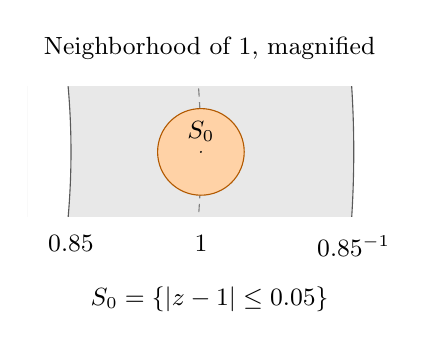
\begin{tikzpicture}[x=11cm,y=11cm,font=\small]
 \begin{scope}
  \clip (0.80,-0.075) rectangle (1.22,0.075);
  \fill[gray!18] (0,0) circle[radius=1.1764706];
  \fill[white] (0,0) circle[radius=0.85];
  \draw[black!65] (0,0) circle[radius=0.85];
  \draw[black!65] (0,0) circle[radius=1.1764706];
  \draw[densely dashed,black!50] (0,0) circle[radius=1];
  \filldraw[fill=orange!35,draw=orange!70!black] (1,0) circle[radius=0.05];
  \fill (1,0) circle[radius=0.0012];
 \end{scope}
 \node at (1.01,0.12) {Neighborhood of $1$, magnified};
 \node[below] at (0.85,-0.085) {$0.85$};
 \node[below] at (1,-0.085) {$1$};
 \node[below] at (1.17647,-0.085) {$0.85^{-1}$};
 \node at (1.01,-0.17) {$S_0=\{|z-1|\leq0.05\}$};
 \node at (1,0.024) {$S_0$};
\end{tikzpicture}
\end{minipage}
\caption{The fixed geometry used in the round-annulus factorization.
The blue disc $p_0(\mathbb D)$ lies in the incoming disc, and the orange
insertion disc lies strictly inside the gray doubled annulus.
The dashed curve is the unit-circle interface.  The transition curves
in the overview are schematic; the magnified panel uses the stated
radii on the central part of the dent.}
\label{fig:fixed-annulus}
\end{figure}

\emph{Factoring the shrinking annulus.}
The map $\gamma_t$ moves the fixed point $a$ to $r$.  We arrange the
remaining incoming boundary by writing
$s\operatorname{id}=\gamma_t\circ p_0\circ b_t$, namely by defining
\[
 b_t=p_0^{-1}\circ\gamma_t^{-1}\circ(s\operatorname{id}).
\]
After doubling, the factor $\gamma_t$ will cancel against its adjoint.
The insertion will then lie between the same fixed factors
$\underline C^*$ and $\underline C$, with only the contractions
$\underline b_t^*$ and $\underline b_t$ outside them.

The disc $\gamma_t^{-1}(s\mathbb D)$ has real diameter with endpoints
$-(s+t)/(1+st)>-1$ and $1/2$.  It lies strictly in $p_0(\mathbb D)$,
so $b_t$ is a strict Möbius disc embedding.  Its covered univalent lift
is a contraction, whereas the lift of $\gamma_t$ is unitary.  Choose
these lifts so that
\begin{equation}\label{eq:round-factorization}
 s^{L_0}=\underline\gamma_t\,
          \underline A_*\underline C\,\underline b_t
\end{equation}
is the standard round-annulus lift.  This is an equality in the covered
univalent semigroup, whose inclusion lifts to
$\widetilde{\operatorname{Ann}}_c$
\cite[Section~4.2]{HTVOA}: the Virasoro cocycle vanishes on the
univalent subalgebra, so this lift introduces no scalar ambiguity.
Any winding adjustment acts unitarily.

Consider the insertion coordinate
$p_t(\zeta)=\gamma_t^{-1}(r+q\zeta)$.  The identities
\[
 1-tr=\frac{1-t^2}{1+ta},\qquad
 \frac{q}{1-tr}=\frac{2(1-a^2)}{t+a}<0.000401,
\]
and
\[
 \gamma_t^{-1}(r+h)-a
   =\frac{(1-t^2)h}{(1-tr)(1-tr-th)}
\]
show, for $|h|\leq q$, that
\[
 |\gamma_t^{-1}(r+h)-a|
  \leq\frac{2(0.000401)}{1-0.000401}<0.000803.
\]
Consequently $p_t(\mathbb D)\subset\mathring S_0$ for every $t$.
The map has no pole there.  Also $s>t$, so the pole $1/t$ of
$\gamma_t^{-1}$ is outside the round annulus with outer radius $1/s$.
Since $\gamma_t$ commutes with reflection in the unit circle, we may
double \eqref{eq:round-factorization}, carrying along the insertion.
The unitary factors cancel, and gluing gives the exact operator identity
\begin{equation}\label{eq:round-doubled}
 A_{1/s,s,N}[(q^{L_0}v)(r)]
 =\underline b_{t,N}^{*}\underline C_N^{*}
    (\underline A_*^\dagger\underline A_*)_N[(p_t)_*v(0)]
    \underline C_N\underline b_{t,N}.
\end{equation}
\emph{The uniform bound.}
Lemma~\ref{lem:fixed-disc} bounds the middle factor by a fixed constant
times $\|v\|$.  Thus the right side has norm at most
$C_{\widehat A_*,S_0}\|\underline C_N\|^2\|v\|$.
In particular, no radius-dependent comparison scalar is introduced.

Finally,
\[
 \frac{1-s}{1-r}
 =5000\frac{1+ta}{1+t/2},
\]
which proves \eqref{eq:round-comparable}.
\end{proof}

\subsection{Transport forms and infinite insertion states}

Recall from \eqref{eq:creation} that, for a unitary module $M$, the creation and annihilation intertwiners are
\[
 \mathcal Y_M^+(a,z)v=e^{zL_{-1}}Y^M(v,-z)a,
 \qquad \mathcal Y_M^-=(\mathcal Y_M^+)^\dagger.
\]
Their types are respectively $\binom{M}{M\,V}$ and
$\binom{V}{\bar M\,M}$.  The charge transform \eqref{eq:theta-convention},
for a complex coordinate with a chosen logarithm, is
\[
 \theta_{\bar z}a
   =e^{\bar zL_1}e^{i\pi L_0}\bar z^{-2L_0}\bar a,
\]
using the conjugate logarithm at $\bar z$.
For unitary modules $M,N$, define the diagonal transport form by
\begin{equation}\label{eq:transport-form}
 \mathfrak t_z^{M,N}(a\otimes b,a'\otimes b')
 =\big\langle
 Y^N\big(\mathcal Y_M^-(\theta_{\bar z}a',
                         \bar z^{-1}-z)a,z\big)b,b'\big\rangle.
\end{equation}
We use this for $0<|z|<1$ and $|z|>|z|^{-1}-|z|$.
At positive real $z$ all positive-coordinate logarithms are real;
on a rotated diagonal the two insertion coordinates have the same
argument and the reflected logarithm is the conjugate one.  The form
is linear in its first entry.

Regularity gives absolute convergence of these matrix coefficients.
More precisely, the ordinary intertwiners between unitary modules have
Hilbert-space values at $0<|z|<1$, with branchwise norm holomorphy
\cite[Definition~2.8, Lemma~2.9 and Proposition~3.11]{TenerFusion}.
Creation satisfies the identity
\begin{equation}\label{eq:creation-transport}
 \mathfrak t_z^{M,V}(a\otimes b,a'\otimes b')
   =\langle\mathcal Y_M^+(a,z)b,
                  \mathcal Y_M^+(a',z)b'\rangle
\end{equation}
without assuming energy bounds, integration of $M$, or positivity of
general fusion forms \cite[Proposition~3.10]{TenerFusion}.

\begin{lemma}[Hilbert-state insertions]\label{lem:transport-cutoff}
Let $M,N$ be unitary modules, with $N$ already integrated.  For
homogeneous $a,a'\in M$ of weights $d,d'$, set
\[
 u_z=\mathcal Y_M^-(\theta_{\bar z}a',\bar z^{-1}-z)a,
 \qquad \delta=|z|^{-1}-|z|,\qquad q=2\delta.
\]
As $|z|$ tends to one on a fixed branch,
\begin{equation}\label{eq:annulus-hilbert-state}
 q^{-L_0}u_z\in\mathcal H_V,
 \qquad \|q^{-L_0}u_z\|\leq C_{a,a'}\delta^{-d-d'}.
\end{equation}
For a fixed dent with $z$ in its inner collar,
$\widehat A_N[u_z(z)]$ is well defined by norm limits of energy
truncations, belongs to $\pi_I^N(A_V(I))$, and has norm at most
$C\delta^{-d-d'}$.  On $\underline A_N^{-1}N$ in both variables it obeys
\begin{equation}\label{eq:transport-cutoff}
 \langle\widehat A_N[u_z(z)]\xi,\eta\rangle
 =\mathfrak t_z^{M,N}
   (a\otimes\underline A_N\xi,
    a'\otimes\underline A_N\eta).
\end{equation}
For the round annuli of Proposition~\ref{prop:round-annulus}, the same
bound holds with the cutoffs $s^{L_0}$ in both entries and $z=r$.
\end{lemma}

\begin{proof}
Expand $\theta_{\bar z}a'$ into finitely many vectors of weights
$d_j\leq d'$.  Their coefficients are bounded as $|z|$ tends to one.
By $L_0$-covariance, applying $q^{-L_0}$ to each annihilation value
produces the factor $q^{-d_j-d}$ and an annihilation value at modulus
$\delta/q=1/2$.  The latter is a Hilbert-space vector by
\cite[Proposition~3.11]{TenerFusion}; rotations preserve its norm.
This proves \eqref{eq:annulus-hilbert-state}.

Let $P_n$ be the vacuum energy cutoff.  Apply the uniform collar
version of \eqref{eq:fixed-disc-bound} to
$q^{-L_0}(P_n-P_m)u_z$.  It gives
\[
 \|\widehat A_N[(P_n u_z)(z)]
       -\widehat A_N[(P_m u_z)(z)]\|
 \leq C\|q^{-L_0}(P_n-P_m)u_z\|.
\]
Thus these operators converge in norm, with the asserted bound.
Locality and representation transfer persist under that norm limit.
For finite truncations, \eqref{eq:annulus-insertion} applies.
Absolute convergence of the transport iterate identifies its limiting
matrix coefficients on the exact dense preimages, proving
\eqref{eq:transport-cutoff}.  The identical argument using
\eqref{eq:uniform-round} and \eqref{eq:round-insertion} gives the
round-annulus assertion.
\end{proof}

\subsection{Charged modes and bounded boundary smears}

\begin{lemma}[Analytic tools for a dominated intertwiner]
\label{lem:charged-tools}
Let $M,N,K$ be grading-restricted unitary $V$-modules, with $N$ already
strongly integrable, and let $\Phi$ have type $\binom{K}{M\,N}$.
Fix a homogeneous $a\in M$ of weight $d$.  Suppose that, for all
finite-energy $b\in N$ and all diagonal positions sufficiently close
to the unit circle on the branches under consideration,
\begin{equation}\label{eq:transport-domination}
 \|\Phi(a,z)b\|^2
   \leq C_a\mathfrak t_z^{M,N}(a\otimes b,a\otimes b).
\end{equation}
Then $\Phi(a,z)$ has polynomial energy bounds, as do its levelwise
adjoint coefficients.  Its smooth smears and their formal adjoints
preserve the smooth domains continuously.

For every smooth test $f$ supported compactly in an interval $I$ with
a chosen argument, there is a localized radial annulus $\underline A$
with a dent over $\operatorname{supp}f$ such that
\begin{equation}\label{eq:charged-bounded-cutoff}
 T_f=\overline{\Phi(a,f)}\,\underline A_N
       :\mathcal H_N\longrightarrow\mathcal H_K
\end{equation}
is bounded and defined on all of $\mathcal H_N$.
Both $T_f$ and $T_f^*$ preserve smooth vectors in their respective
directions.  Moreover,
\[
 N\subset\operatorname{ran}\underline A_N,
 \qquad \underline A_N^{-1}N\text{ is dense in }\mathcal H_N.
\]
These conclusions apply to $\Phi=\mathcal Y_M^+$ and $N=V$ for every
already unitary $M$, before integrating $M$.
\end{lemma}

\begin{proof}
Lemma~\ref{lem:transport-cutoff} and
Proposition~\ref{prop:round-annulus} give
\begin{equation}\label{eq:charged-radial-estimate}
 \|\Phi(a,r)s^{L_0}b\|
      \leq C(1-r)^{-d}\|b\|,
 \qquad b\in N.
\end{equation}
Write the physical expansion as
$\Phi(a,z)=\sum_\mu\Phi(a)[\mu]z^{-\mu-d}$, so that a coefficient
maps energy $h$ to $h-\mu$.  For $b$ of energy $h$, project
\eqref{eq:charged-radial-estimate} to that output energy.  Fix
$0<\varepsilon_a\leq10^{-4}$ small enough that the transport domination
and the cutoff estimate hold whenever $1-\varepsilon_a\leq r<1$, and choose
\[
 1-r=\frac{\varepsilon_a}{1+h+|\mu|}.
\]
The corresponding $t$ lies in $[0,1)$.  By
\eqref{eq:round-comparable}, $s\geq1/2$ and
$1-s\leq(6667)10^{-4}/(1+h+|\mu|)$.
Since $-\log s\leq2(1-s)$, the factor $s^{-h}$ is uniformly bounded.
The factor $r^{\mu+d}$ is uniformly bounded as well, using $d\geq0$
and $r\geq1-10^{-4}$.  Hence
\begin{equation}\label{eq:charged-mode-estimate}
 \|\Phi(a)[\mu]b\|
     \leq C(1+h+|\mu|)^d\|b\|.
\end{equation}
Distinct input energies have distinct output energies for a fixed
coefficient.  Orthogonality therefore turns this into a polynomial
energy bound on $N$.  Taking adjoints between individual energy spaces
gives the same kind of bound for the adjoint coefficients.  Choose any
integer energy order at least $d$ when an integer order is desired.

On a fixed argument interval, define $\Phi(a,f)$ by smearing its physical
field $z^d\Phi(a,z)$ against $f(e^{i\vartheta})\,d\vartheta/(2\pi)$.
Other smooth weight factors can be absorbed into $f$.  Rapid decay of
Fourier coefficients, \eqref{eq:charged-mode-estimate}, and the energy
shifts show that this smear and its formal adjoint map smooth vectors
continuously to smooth vectors.  For clarity, a target Sobolev seminorm
of order $j$ is bounded by an input seminorm of a fixed higher order,
times a summable series of polynomially weighted Fourier coefficients.
This also shows that finite-energy truncations converge in the graph
norm of the smear.  The closures of the smears defined on finite-energy
and on smooth vectors consequently agree.

Choose $\underline A$ with $\rho<1$ on a neighborhood of
$\operatorname{supp}f$ and with $1-\rho$ compactly supported in $I$.
On the fixed dense subspace $\underline A_N^{-1}N$, consider
\[
 T(z)\xi=\Phi(a,z)\underline A_N\xi.
\]
The localized part of Lemma~\ref{lem:transport-cutoff}, together with
\eqref{eq:transport-domination}, gives a bounded extension satisfying
\begin{equation}\label{eq:charged-collar}
 \|T(z)\|\leq C(1-|z|)^{-d}
\end{equation}
throughout an inner collar over this neighborhood.  Its values on the
dense initial domain are Hilbert-valued holomorphic functions, by
\cite[Lemma~2.9 and Proposition~3.11]{TenerFusion}.
Local uniform boundedness therefore gives operator-norm holomorphy.

For neutral fields, annulus regularization and the Banach-valued
boundary argument appear in \cite[Proposition~8.4 and Lemma~8.5]{HTVOA}.
The charged collar estimate \eqref{eq:charged-collar} supplies the
hypothesis needed here. We spell out the boundary argument.
Put
\[
 F_f(t)=\int f(e^{i\vartheta})e^{id\vartheta}
                         T(te^{i\vartheta})\,\frac{d\vartheta}{2\pi}.
\]
All integrals here use the chosen argument and the compact support of
$f$.  Holomorphy gives $t\partial_tT=-i\partial_\vartheta T$.
After integrating by parts, every radial derivative of order $p$ of
$F_f$ is a finite sum of integrals of $T$ against derivatives of the
fixed smooth test, multiplied by bounded powers of $t^{-1}$.
Thus
\[
 \|F_f^{(p)}(t)\|\leq C_{f,p}(1-t)^{-d}.
\]
Choose an integer $p>d$.  Taylor's integral formula from a fixed
$t_0<1$ expresses $F_f(t)$ as a polynomial plus the integral of
$(t-u)^{p-1}F_f^{(p)}(u)/(p-1)!$.
The norm of the latter integrand is bounded, uniformly for $u\leq t$,
by a constant times $(1-u)^{p-1-d}$, which is integrable at one.
Dominated convergence proves that $F_f(t)$ has an operator-norm limit
$T_f$ as $t$ tends to one.

On $\underline A_N^{-1}N$, the mode expansion and its polynomial bounds
identify this limit with $\Phi(a,f)\underline A_N$.
For arbitrary $\xi\in\mathcal H_N$, approximate $\xi$ by
$\xi_j\in\underline A_N^{-1}N$.  Then
$\underline A_N\xi_j\to\underline A_N\xi$ and
$T_f\xi_j\to T_f\xi$.  Closedness of the smeared field proves
\eqref{eq:charged-bounded-cutoff} on all of $\mathcal H_N$.
Lemma~\ref{lem:annulus-range} supplies the asserted range and density.

The product in \eqref{eq:charged-bounded-cutoff} preserves smooth
vectors, since both its factors do.  If $\Phi(a,f)^\dagger$ denotes
the formal adjoint smear, then every smooth target vector $\eta$
belongs to the adjoint domain of $\overline{\Phi(a,f)}$, and
\[
 T_f^*\eta=\underline A_N^*\Phi(a,f)^\dagger\eta.
\]
Indeed this equality follows by pairing with the dense finite-energy
core and using the adjoint coefficient bounds.  The right side is
smooth: the formal adjoint smear preserves smooth vectors and the
fixed annulus adjoint preserves every Sobolev space.  This proves the
remaining domain assertion.  Finally,
\eqref{eq:creation-transport} supplies
\eqref{eq:transport-domination} with constant one for creation, with
the vacuum as its integrated source.
\end{proof}
